\documentclass[thesis.tex]{subfiles}

\begin{document}

\chapter{Evaluation}\label{chap:eva}

This chapter contains the results of the experiments from the different strategies and methods as discussed in \autoref{chap:main}. The experiment shall show if the postulated SpeedCam approach achieves the goals (\autoref{sec:intro:goals}). At first, it describes the test environment so that the experiment is repeatable and the results are verifiable. Then it list the different experiment configuration and lastly their results, which will be interpreted and discussed. The following \autoref{chap:concl} draws the conclusion of these results.

\section{Test environment}

There are two different used test environments to validate the theses.
The first one is a local virtual machine of Ubuntu 16.04 LTS under a Windows 10 host. The host is an i7-6700K with 16GB DDR-2133. The image is placed on a SSD 850 EVO. The virtual machine can use 4GB of RAM and 4 logical cores. Inside this VM is a virtual network running the default topology as shown in \autoref{fig:eva:defaultTopo}. The installation process is the same as described in the SCION readme.me\footnote{\url{https://github.com/scionproto/scion/blob/master/README.md}, 07.04.2018}. Each component of the virtual network is running as a own process and interact with each other.

\begin{figure}
	\centering
	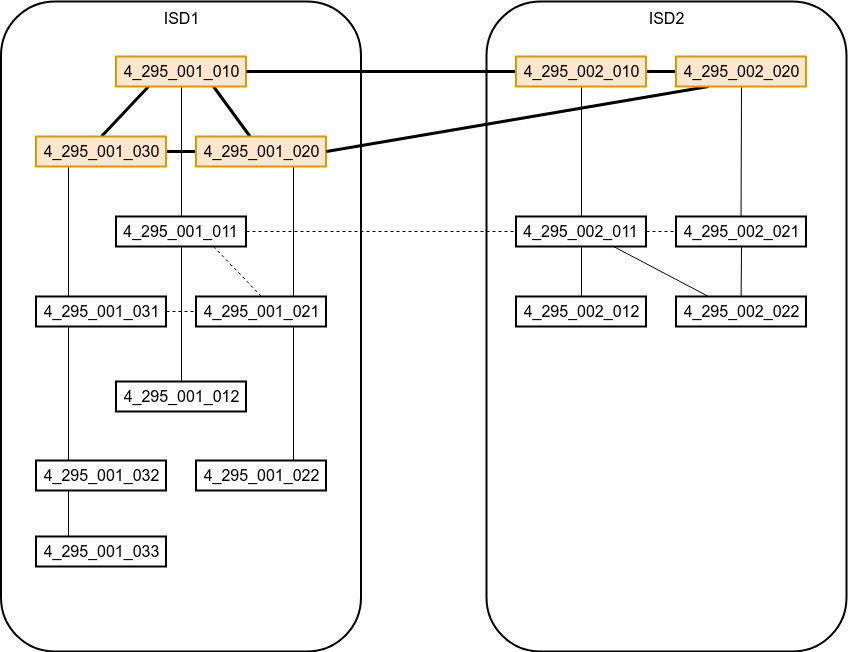
\includegraphics[height=8cm]{default_topo}
	\caption*{\tiny{\url{https://github.com/scionproto/scion/blob/master/doc/fig/default_topo.png}, 07.04.2018}}
	\caption{Default topology}
	\label{fig:eva:defaultTopo}
\end{figure}

The second environment is that of SCIONLab in its current state. A part of this network is seen in \autoref{fig:eva:scionLabTopo}, which is the topology after a few exploration episodes. It does not represent the complete topology, only the current observed one. The inspector program is running on the same machine as the SCPB, while the scripts for information about border router interfaces and path server requests are running on different machines. The inspectors machine is a virtual machine \todo{Specs dieser virtuellen maschine erfragen}

\begin{figure}
	\centering
	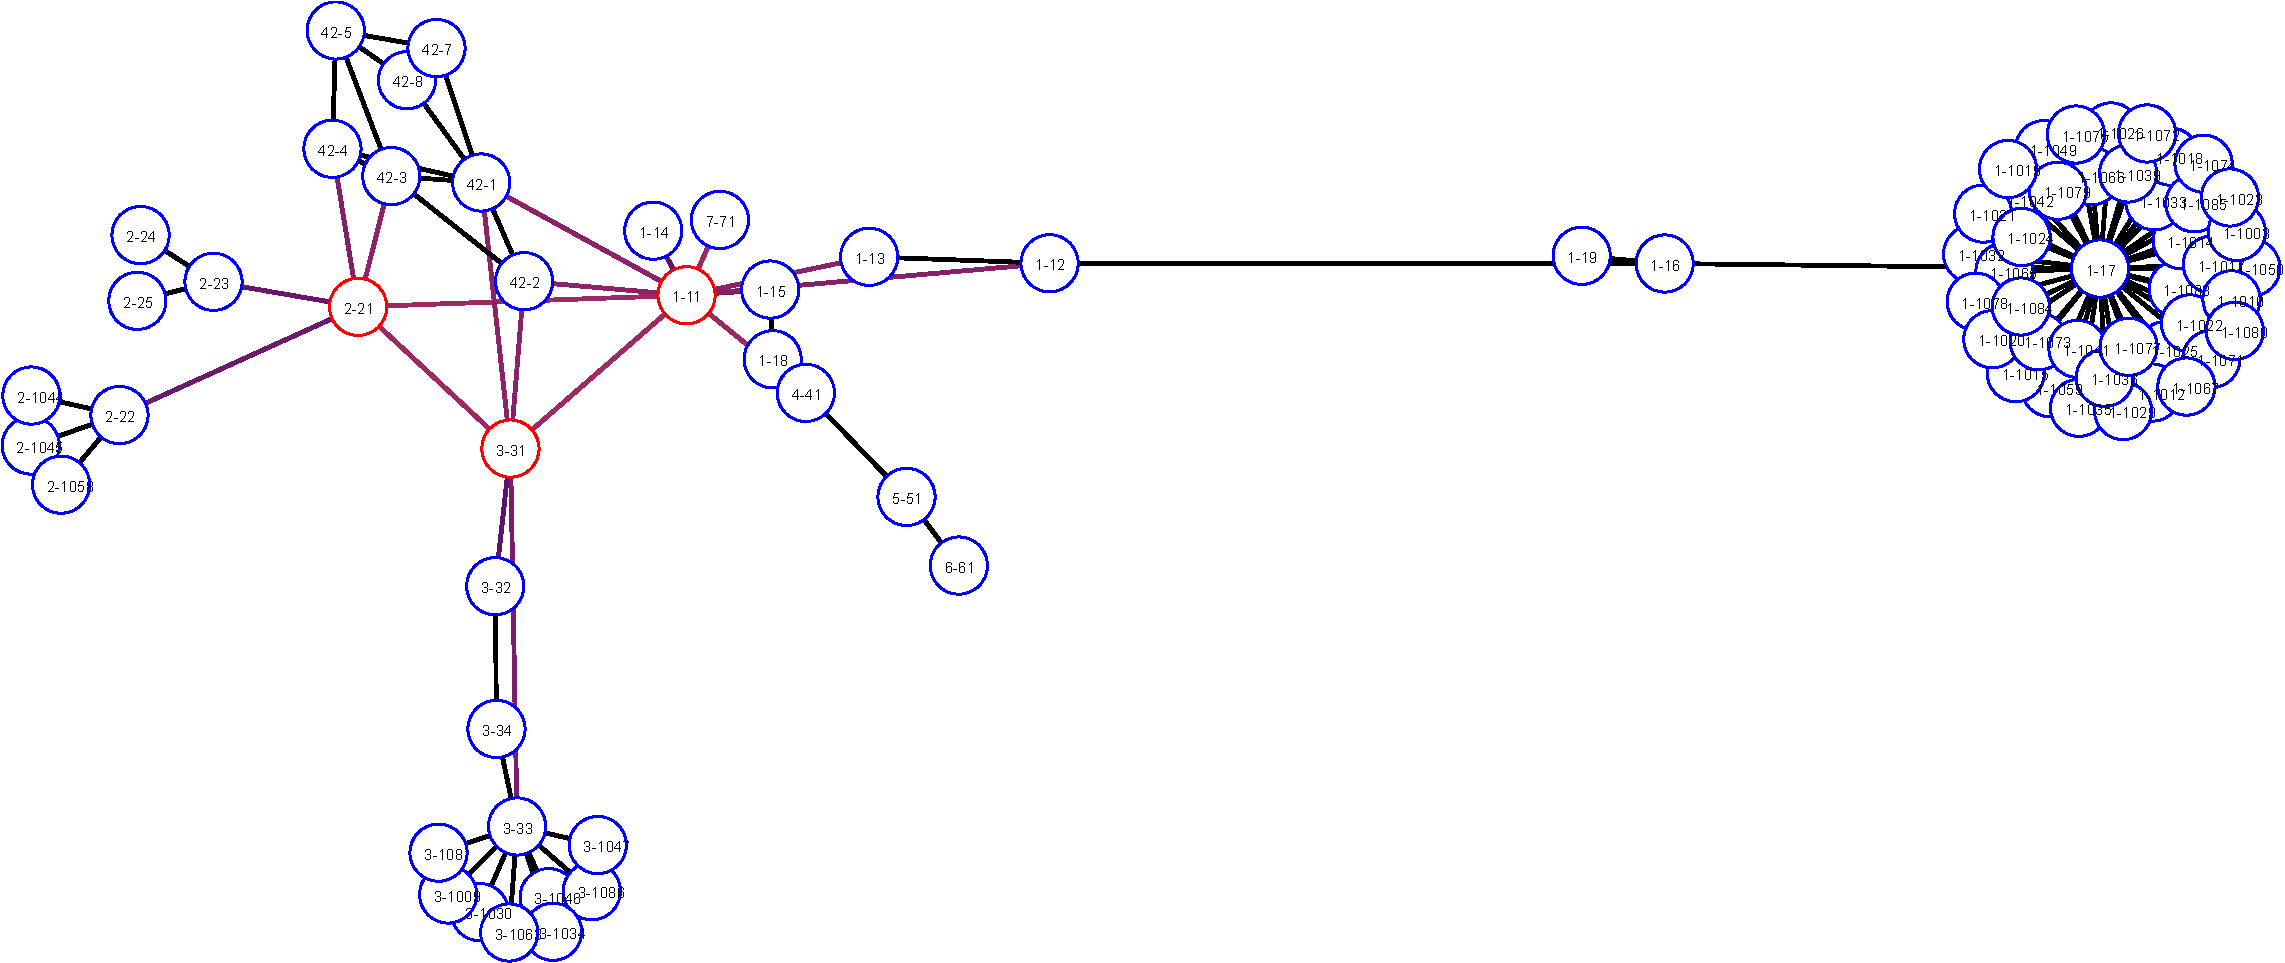
\includegraphics[width=.9\linewidth]{scionLabTopology.pdf}
	\caption{Part of SCIONLab topology}
	\label{fig:eva:scionLabTopo}
\end{figure}

\subfilebib % Makes bibliography available when compiling as subfile
\end{document}